\documentclass{exam}
\usepackage[utf8]{inputenc}
\usepackage{lmodern}
\usepackage{microtype}

% \usepackage[parfill]{parskip}
\usepackage[dvipsnames]{xcolor}
\usepackage{amsmath}
\usepackage{amsfonts}
\usepackage{amsthm}
\usepackage{siunitx}
\DeclareSIUnit\year{yr}
\DeclareSIUnit\foot{ft}
\DeclareSIUnit\litre{\liter}

\usepackage{skull}

\usepackage{pgfplots}
\usepgfplotslibrary{polar}
\pgfplotsset{compat=1.11}
\usepgfplotslibrary{statistics}
\usepackage{graphicx}
\usepackage{sidecap}
\sidecaptionvpos{figure}{c}
\usepackage{float}
\usepackage{gensymb}
\usepackage{tkz-euclide}
\usetkzobj{all}
\usepackage{commath}
\usepackage{hyperref}
\usepackage{enumitem}
\usepackage{wasysym}
\usepackage{multicol}
\usepackage{mathtools}
\usepackage{tcolorbox}
\usepackage{tabularx}
\usepackage[version=4]{mhchem}
\usepackage{changepage}
\usepackage{listings}
\lstset{basicstyle=\ttfamily\linespread{0.8}\small}

\renewcommand*{\thefootnote}{\fnsymbol{footnote}}

\newtheorem*{thm}{Theorem}
\newtheorem*{iden}{Identity}
\newtheorem*{lemma}{Lemma}
\newtheorem{obs}{Observation}
\theoremstyle{definition}
\newtheorem*{defn}{Definition}
\newtheorem*{ex}{Example}
\newtheorem{con}{Construction}
\newtheorem*{alg}{Algorithm}

\newtheoremstyle{break}
  {\topsep}{\topsep}%
  {\itshape}{}%
  {\bfseries}{}%
  {\newline}{}%
\theoremstyle{break}
\newtheorem*{bthm}{Theorem}

% russian integral
\usepackage{scalerel}
\DeclareMathOperator*{\rint}{\scalerel*{\rotatebox{17}{$\!\int\!$}}{\int}}

% \DeclareMathOperator*{\rint}{\int}

\pgfplotsset{vasymptote/.style={
    before end axis/.append code={
        \draw[densely dashed] ({rel axis cs:0,0} -| {axis cs:#1,0})
        -- ({rel axis cs:0,1} -| {axis cs:#1,0});
    }
}}

% \pointsinrightmargin
\boxedpoints
\pointname{}

\newcommand{\questioA}{\question[\texttt{\textbf{\color{Cerulean} A}}]}
\newcommand{\questioM}{\question[\texttt{\textbf{\color{PineGreen} M}}]}
\newcommand{\questioE}{\question[\texttt{\textbf{\color{WildStrawberry} E}}]}
\newcommand{\questioS}{\question[\texttt{\textbf{\color{Goldenrod} S}}]}
\newcommand{\questioO}{\question[\texttt{\textbf{\color{BurntOrange} O}}]}

\newcommand{\parA}{\part[\texttt{\textbf{\color{Cerulean} A}}]}
\newcommand{\parM}{\part[\texttt{\textbf{\color{PineGreen} M}}]}
\newcommand{\parE}{\part[\texttt{\textbf{\color{WildStrawberry} E}}]}
\newcommand{\parS}{\part[\texttt{\textbf{\color{Goldenrod} S}}]}
\newcommand{\parO}{\part[\texttt{\textbf{\color{BurntOrange} O}}]}

\newcommand{\subparA}{\subpart[\texttt{\textbf{\color{Cerulean} A}}]}
\newcommand{\subparM}{\subpart[\texttt{\textbf{\color{PineGreen} M}}]}
\newcommand{\subparE}{\subpart[\texttt{\textbf{\color{WildStrawberry} E}}]}
\newcommand{\subparS}{\subpart[\texttt{\textbf{\color{Goldenrod} S}}]}
\newcommand{\subparO}{\subpart[\texttt{\textbf{\color{BurntOrange} O}}]}

\newcommand{\mainHeader}[2]{\section*{NCEA Level 2 Mathematics\\#1. #2}}
\newcommand{\mainHeaderHw}[2]{\section*{NCEA Level 2 Mathematics (Homework)\\#1. #2}}
\newcommand{\seealso}[1]{\begin{center}\emph{See also #1.}\end{center}}
\newcommand{\drills}[1]{\begin{center}\emph{Drill problems: #1.}\end{center}}
\newcommand{\basedon}[1]{\begin{center}\emph{Notes largely based on #1.}\end{center}}

\begin{document}

\section*{NCEA Level 3 Calculus (Differentiation)\\Prior Revision: Functions}

\begin{center}
  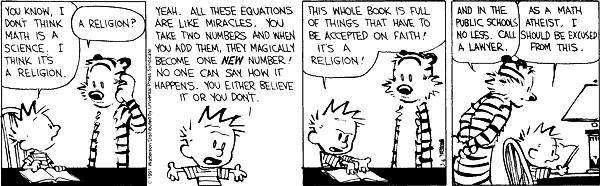
\includegraphics[width=0.8\textwidth]{hobbes}
\end{center}

\subsection*{Introduction to the Notes}
\subsubsection*{Mathematical Prerequisites}
There are a number of things from Level 2 Mathematics that students should be
comfortable with; generally, I assume in these notes a vague merit-level understanding
of the core level 2 standards (by which I mean, the reader should be comfortable solving
achieved level problems without guidance and have some idea how to approach more difficult
problems):
\begin{itemize}
  \item Level 2 Algebra: All material on quadratics (factorising, solving, discriminants), logs and exponents.
  \item Level 2 Calculus: Basic differentiation, geometric meaning of derivative (in particular, integration is \textit{not} assumed)
  \item Level 2 Graphing: Recognising $ x-$/$ y-$shift of general functions, slope-intercept and point-slope form of linear equations,
                          recognising period/frequency/amplitude/$ x-$/$ y-$shift from a trig function.
  \item Level 2 Trigonometry: Trig ratios, the Pythagorean theorem.
  \item Level 2 Simultaneous Equations: Solving linear and quadratic simultaneous equations.
  \item Level 2 Co-ordinate Geometry: Distances and linear equations.
\end{itemize}

Further into the notes, I also touch a bit on concepts covered in some of the other Level 3 standards,
but not in so much detail that they need to be covered first:
\begin{itemize}
  \item Level 3 Conics: Recognising forms from equations.
  \item Level 3 Algebra: Surds.
  \item Level 3 Trigonometry: Solving trig equations (including general solutions), reciprocal trig functions, use
                              of trig identities (this latter mainly for E/S/OS-style integration problems).
\end{itemize}
In particular, no knowledge of complex algebra is assumed (or used) anywhere in the notes.

No knowledge from any L2 or L3 statistics standards is assumed.

\subsubsection*{A Note on Problem Difficulty}
One of the main goals for these notes is that they should be useful for students at all levels, from A to OS. Accordingly, the
problems each week range from simple (most students should be able to just write down an answer without thinking too hard) to
extremely non-trivial (it took \textbf{me} a while to work the problem, and I know this material quite well). If you can't do
a problem, the best thing to do is to move on and come back to it --- the problems don't always increase in difficulty. Of course,
it is important to do a good number of problems \textbf{including some difficult ones}; you're not under exam conditions here
and you're going to get an awful lot more out of a hard problem than an easy one!

I have marked the problems in the weekly worksheets (\textbf{not} the homework) with symbols relating vaguely to difficulty:

\begin{center}
\texttt{\textbf{\color{Cerulean} A}}
\texttt{\textbf{\color{PineGreen} M}}
\texttt{\textbf{\color{WildStrawberry} E}}
\texttt{\textbf{\color{Goldenrod} S}}
\texttt{\textbf{\color{BurntOrange} O}}
\end{center}

However, these are for my own reference and should not be taken to be accurate with respect to actual examinations.

\subsubsection*{A Note on the Textbook}
Many problems are taken from a couple of places:
\begin{itemize}
  \item Stewart's Calculus (the current trendy textbook)
  \item Anton's Calculus (the old trendy textbook)
  \item Spivak's Calculus (the textbook you should use)
  \item University of Canterbury MATH199 lecture notes and problem sets
  \item Old NCEA/Scholarship exams
\end{itemize}
Most textbooks cover all the relevant material in the first few chapters (the first five or so in Stewart).

\subsubsection*{Homework}
Every week has an associated homework sheet with a page of reading (five minutes or so) and a few questions (generally all
pretty straightforward, but there is often a challenge question on there to keep you occupied).

I cannot emphasise enough how important it is to \textbf{do the homework}.

\subsubsection*{How to Read Mathematics}
\begin{center}
  \textit{So we shall now explain how to read the book. The right way is to put it on your desk in the day, below your pillow at night, devoting yourself to the reading, and solving the exercises till you know it by heart. Unfortunately, I suspect the reader is looking for advice on how not to read, i.e. what to skip, and even better, how to read only some isolated highlights.}\\ - Saharon Shelah, `Classification Theory and the Number of Non-Isomorphic Models'
\end{center}

A major part of Level 3 Mathematics is preparation for university-level study in pure mathematics or the hard or soft sciences. As such, this
year we begin to expose you to some `real mathematics' --- not just the watered-down calculation and computation you've been doing since intermediate,
but a real journey of discovery through one of humanity's great fields of human experience. I guarantee that at primary school you enjoyed
this kind of mathematics --- for example, consider the non-obvious fact that $ 3 \times 5 = 5 \times 3 $. Next year you will learn that there are
some objects which do not have this property (commutativity).

There are a lot of definitions and theorems, but they allow us to capture our intuition of mathematical objects, their behaviour, and their beauty
in a more precise (and more correct) sense. It is important to read slowly and understand the statements as you go, as every piece strengthens the
whole. I do not tend to repeat myself, so often you will find statements from earlier used later without comment.

\textbf{Recommended reading for the interested}: Paul Lockhart's `A Mathematician's Lament'.

\clearpage
\subsection*{Welcome to Calculus}
\subsubsection* {What is Calculus?}
Calculus is the study of:
\begin{itemize}
  \item Continuous change.
  \item Slope, area, and volume.
  \item Functions and relationships.
\end{itemize}

It has applications in:
\begin{itemize}
  \item Physics and chemistry.
  \item Probability theory.
  \item Population theory.
  \item Economics (I am assured).
\end{itemize}

In pure mathematics, calculus can be seen as the computational side of a pretty
subject called \textbf{real analysis}.

\subsubsection*{Revision of Functions}
The most fundamental concept in calculus is that of a \textit{function}.

\begin{defn}[Function]
  A function is a something which takes a set of things (for example, the real numbers $ \mathbb{R} $) and assigns
  to each one exactly one thing (which could be the same or different).
\end{defn}

\begin{ex}
  The map which takes a number $ x $ and spits out $ x^2 $ is a function --- for every input, there is exactly one output. If
  we \textit{graph} this function, we plot its input on the $ x-$axis and its output on the $ y-$axis and obtain a parabola.
\end{ex}

\begin{ex}
  The curve graphed below is \textit{not} a function, since for some inputs (like 1) it has more than one output. We can check this
  by drawing vertical lines along the function, like that pictured: if a graph is a function, no vertical line can ever cross the curve
  more than once (this is the \textit{vertical-line test}).

  \begin{center}
    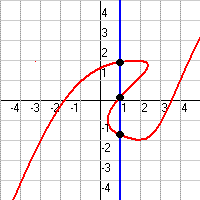
\includegraphics[width=0.3\textwidth]{linetest}
  \end{center}
\end{ex}

\begin{ex}
  The map $ f : x \mapsto \sin x $ is a function. We could also define it by `the function $ f $ such that $ f(x) = \sin x $'.
  This function $ f $ can only produce numbers between $1$ and $-1$; we say that its \textit{range} is the interval from $ -1 $ to 1.
\end{ex}

\begin{ex}
  The map $ \iota : x \mapsto x $ is a function, called the \textit{identity function}.
\end{ex}

\begin{ex}
  The map $ \ln x $ is a function, but it is only defined when $ x > 0 $: we say that its \textit{domain} is the positive real numbers.
\end{ex}

\clearpage
\begin{ex}
  Some more non-examples:

  \begin{center}
    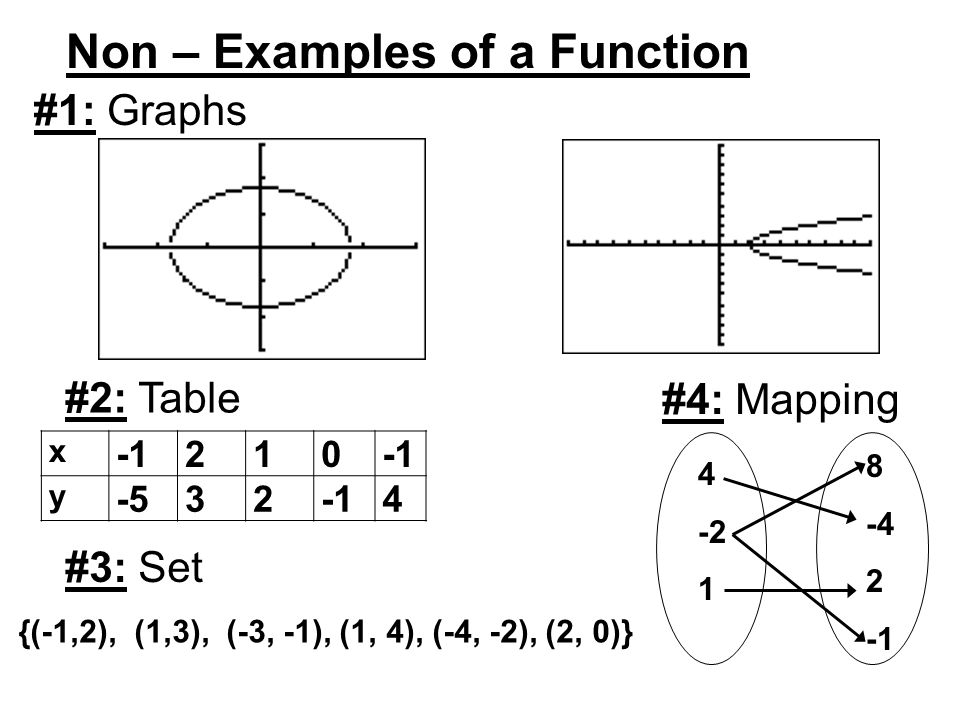
\includegraphics[width=0.5\textwidth]{notfunction}
  \end{center}
\end{ex}

\subsection*{Questions}
\begin{questions}
  \question Which of the following are functions?
    \begin{parts}
      \part $ E(x) = 2^x $
      \part $ \phi : x \mapsto \frac{2}{x} $
      \part The thing which maps every person to their youngest sibling.
      \part The thing which sends every person to their youngest sibling that isn't themself.
      \part $ x \mapsto \lfloor x \rfloor $ (the floor map).
      \part The relation that sends every person to their age.
    \end{parts}
  \question I will define two functions, $ \varphi $ and $ \vartheta $, as follows:
            \begin{displaymath}
              \varphi(x) = 2x - 7, \qquad \vartheta(\zeta) = \frac{1}{7}(14\zeta - 49).
            \end{displaymath}
            Explain why these functions are equal.
  \question If $ f(x) = x^2 + x $, find:
    \begin{parts}
      \item $ f(1) $
      \item $ f(y) $
      \item $ f(x + h) $
    \end{parts}
  \question Find the distance between $ (-3, 4) $ and $ (2, 1) $.
  \question Three sides of a triangle are have lengths 8, 15, and 17.
    \begin{parts}
      \part Show that the triangle is right-angled.
      \part Find the other two angles.
    \end{parts}
  \question Factorise and solve $ x^2 - 3x + 2 = 0 $.
  \question How many \textbf{lines} are there through the point $ (2,3) $ and the origin? Give the equations of all such lines.
  \question Find the slope of the line $ 4x + 3y + 2 = 0 $.
  \question Find the solution to the following linear system:
            \begin{align*}
              2x + y &= 7\\
              3x - y &= 8
            \end{align*}
  \question How many (real) solutions does $ x^2 + 4x + 1 $ have?
  \question Draw $ \sin(x) $, $ \cos(x) $, $ \tan(x) $, $ \exp(x) $, and $ \ln(x) $.
  \question How many solutions does $ \cos (3\pi x + 1) = 2 $ have?
  \question How many solutions does $ \sin (3x) = \frac{1}{3} $ have?
\end{questions}

\end{document}
